\documentclass[authoryearcitations]{UoYCSproject}
\usepackage{graphicx}
\graphicspath{ {images/} }
\author{David M. Taylor}
\title{Road Safety Advisory System}
\date{Version 0.2, 2014-March-17}
\supervisor{Dr. Radu Calinescu}
\BEng
\wordcount{xxx}


\abstract{ ... }


\acknowledgements{ ... }

\begin{document}
\maketitle
\listoffigures
\listoftables
\renewcommand*{\lstlistlistingname}{List of Listings}
\lstlistoflistings

\cleardoublepage
\label{sec:start}
\thispagestyle{empty}\cleardoublepage

\chapter{Introduction}

\section{Project Area and Motivation}

It is envisaged that open data, i.e. data that can be freely used and redistributed by anyone, released by governments will lead to major social and economic advances. Deloitte, one of the largest professional services firms in the world, believes that every business should have a strategy to exploit the growing estate of open data \citep{DeloitteAnalytics2012}. Furthermore, in the Open Data Charter of 18 June 2013, it is acknowledged that the use of open data can spur economic growth \citep{CabinetOffice2013}. The Open Data charter states that members of G8 are committed to releasing open data in order to create more accountable, responsive, and effective governments and businesses. Open data increases transparency about what government and businesses are doing, which promotes accountability and good governance.

The Open Data Charter also states that "freely-available government data can be used in innovative ways to create useful tools and products that help people navigate modern life more easily". It is this use of open data that forms the motivation for this project. There are already a large number of applications available that make use of various open data sets. The \textit{data.gov.uk} website has a catalogue of 350+ applications \citep{Data.go}, each of which take open datasets and make the data a usable resource for the general public. 

Several of these applications make use of road safety data published by the UK Department for Transport. These applications all have key limitations that impact the usefulness of the application for the general public and the open data community. For example, they are not capable of highlighting accident hotspots on a user specified route. Additionally, the source code behind these applications isn't open source, so there is little help available for people looking to build their own applications.


\section{Project Aims and Objectives}

The principle aim of this project is to develop and evaluate an application that allows a user to view and interact with open data via an interactive map. More specifically, I aim to build a web application that uses road safety data provided by the UK Department for Transport, in order to warn road users about accident hotspots.

I'm also aiming to build a framework that can be followed by other developers in the future, in order to simplify and encourage the development of similar applications. This will hopefully lead to more open data sets being used for the benefit of the general public.

\section{Statement of Ethics}

All data and technologies used within this project are open source. No human participation is involved so there are no serious ethical concerns.

\section{Report Structure}
The remainder of this report is organised as follows:

Chapter 2 provides a background of open data, and a review of the literature associated with the open data movement. It also covers more general areas of software development, including web application technologies, software engineering methodologies and usability of interactive applications.

Chapter 3 describes the functional and non-functional requirements gathered to develop the road safety advisory system.

Chapter 4 presents the system architecture, development process, technology overview and interface designs. All design decisions made will be explained in this chapter.

Chapter 5 describes the components created and techniques used during the implementation phase. It also describes the testing process followed, and the outcomes of testing.

Chapter 6 provides an evaluation of the application. This includes a discussion of which requirements were met, along with an analysis of the usability, maintainability and limitations of the application.

Chapter 7 summarises the achievements of the project and presents suggestions for future work in this area.

\chapter{Literature Review}

\section{Open Data}

The formal definition of open data states that "open data is data that can be freely used, modified, and shared by anyone for any purpose" \citep{OpenKnowledge}. The release of open datasets by governments is becoming increasingly popular as the benefits become more apparent.

In this section of the report, I will look at the history of the open data movement, benefits and challenges that it introduces, applications using road safety data, and research areas involving open data.

\subsection{The Open Data Movement}

The origins of the open data movement can be traced back as far as 1942, when Robert King Merton explained the importance of making research results freely accessible to all \citep{Chignard2013}. The term open data wasn't coined until 1995, when an American scientific agency used it in reference to a complete and open exchange of scientific information between countries. Researchers were the first to recognise the benefits of sharing data in this manner. This concept of sharing data, along with the growing popularity of open source software led to the foundation of open data.

The open data movement in the UK started to pick up momentum as early as 2006, when The Guardian launched its "Free Our Data" campaign \citep{GuardianTechnology2006}. This campaign called for raw data gathered by Ordnance Survey to be made freely available for reuse by individuals and companies. This campaign partially achieved its goal when, on 1 April 2010, Ordnance Survey released the brand OS OpenData \citep{OrdnanceSurveyteam2010}. The campaign has since continued, with the aim of making more data publicly available. 

In 2007, a meeting was held in Sebastopol, USA, with the aim of defining the concept of open public data and have it adopted by the US presidential candidates. This meeting was hugely successful, and ultimately led to Barack Obama signing two presidential memoranda concerning Open Data the following year. 

In 2009, \textit{data.gov} was launched, with the objective of increasing public access to high value, machine readable datasets. Later in the year, the White House issued an Open Government Directive requiring federal agencies to take immediate, specific steps to achieve key milestones in transparency, participation, and collaboration \citep{Orszag2009}. This required that all agencies post at least three high-value data sets online and register them on \textit{data.gov}.

In 2009, the UK Prime Minister appointed the founder of the World Wide Web, Sir Tim Berners-Lee, as expert advisor on public information delivery \citep{CabinetOffice2009}. Berners-Lee was asked to oversee the work to create a single point of access for government held public data and develop proposals to extend access to data from the wider public sector, including selecting and implementing common standards. This work led to the launch of \textit{data.gov.uk} in January 2010. On launch the site contained 2,500 datasets, and it now contains over 19,500 from areas as diverse as transport, health, and the economy. This increase demonstrates the open data push that has taken place over the last few years in the UK, as the government strives to improve its openness.

The Open Government Partnership was launched in September 2011, with the aim of "securing concrete commitments from governments to promote transparency, empower citizens, fight corruption, and harness new technologies to strengthen governance" \citep{OpenGovernmentPartnership}. From just eight founding governments, there are now 65 participating countries. These countries have made over 1,000 commitments to make their governments more open and accountable.

The Open Data Institute (ODI) was founded by Sir Tim Berners-Lee and Nigel Shadbolt in 2012. The ODI is a not-for-profit organisation, dedicated to promoting Open Data. The ODI aims to "catalyse the evolution of open data culture to create economic, environmental, and social value" \citep{TheOpenDataInstitute}. They now have over 100 members who demonstrate the values of open data to their business and their customers. In the last year, the ODI have trained over 700 people and held over 80 events. They have made considerable effort in promoting the value of open data across the world; there are now 22 'ODI Nodes' in 15 countries \citep{TheOpenDataInstitute2015a}.

On 9 May 2013, Barack Obama signed an executive order \citep{TheWhiteHouse-OfficeofthePressSecretary2013} that made open and machine-readable data the new default for government information. The US government has launched a number of open data initiatives aimed at scaling up open data efforts across the Health, Energy, Climate, Education, Finance, Public Safety, and Global Development sectors. The number of available datasets on \textit{data.gov} has grown rapidly in recent years, with over 130,000 now available. This shows that, like the UK, the US administration has taken large steps to improve its openness.

\subsection{Benefits and Challenges of Using Open Data}


%Tim O'Reilly played a big role in the Sebastopol meeting and the open data movement in the US as a whole. He has since written about how government can improve by embracing open data.  He believes that government can learn from open-source software, by becoming "an open platform that allows people inside and outside government to innovate" \citep{OReilly2011}. 


\subsection{Uses of Road Safety Data}

Before developing my own application, I will carry out a study of existing web applications that use road safety data. My aim is to identify common characteristics, principles and components that can be reused in my application. I will also look at the limitations of these applications, so that I can look to improve on them.

The applications described below were identified as closest in type and/or purpose to this project.
 
Crash Map \citep{crashmap} displays UK road accidents on an interactive map. You can search for a location, and filter the accident data used according to severity, casualty types, and year of accident (2005-2013). The application plots all accidents found within the current bounding box, with the colour of each marker signifying the severity (see \autoref{fig:crashmap}). If there is a large number of results, you must zoom in further in order for them to be displayed on the map. You can click on a marker for any accident in order to see more information, and then you can request a detailed report for that accident (there is a charge for this service).

The application uses the Google Maps API, but there is no further information about technologies used. The code isn't open source, so there is no benefit to other developers who are looking to build similar applications using open data. 

Crash Map is useful for viewing where accidents have occurred within a specific area, and finding detailed information about them. However, it is reasonable to assume that a user may be more interested in finding out about accidents on a particular route from one location to another, rather than looking at an area. Crash Map is incapable of analysing the data in this way, which is a major limitation.

\begin{figure}
	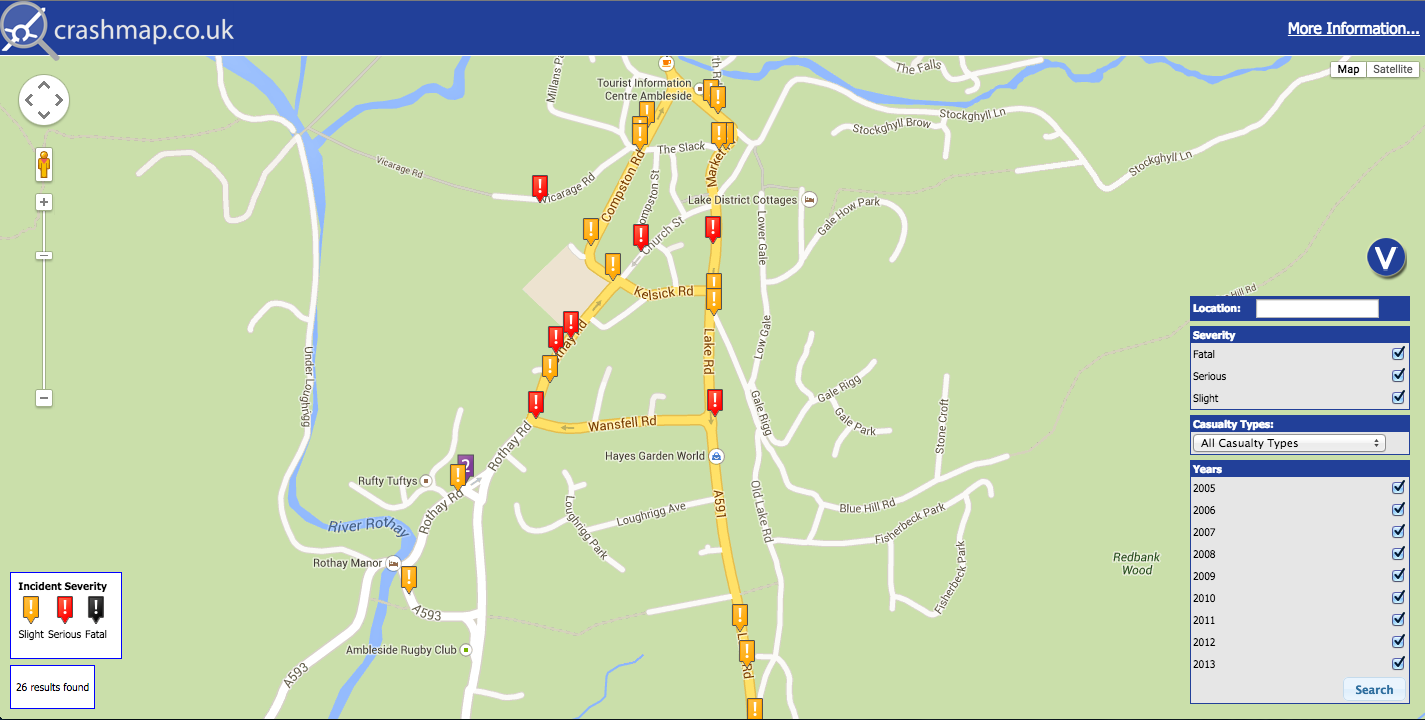
\includegraphics[scale=0.3]{crashmap}
	\caption{Crash Map application}
	\label{fig:crashmap}
\end{figure}

Collision Map \citep{DepartmentforTransport} is similar in purpose to Crash Map. It displays the location of accidents on an interactive map, and also has filters that can be used, including severity, casualty age band and vehicle type (see \autoref{fig:collisionmap}). It differs to Crash Map in that you must select a local highway authority rather than searching for a location or using the map to find it. Clusters of accidents are displayed as one marker on the map, with a number representing how many accidents are in that area. You can reveal the exact location of each accident by zooming in further.

Collision map has several useful features, but has similar limitations to Crash Map. The main advantage of this application is the grouping of accidents to signify hotspots. This makes it very easy to look at an area and see where the most accidents have occurred. A disadvantage in comparison to Crash Map is that you can only use accident data for one year in any search. Like Crash Map, it also lacks the capability of analysing particular routes. This becomes particularly difficult if a route passes through more than one highway authority as you would need to change the search parameters. 

\begin{figure}
	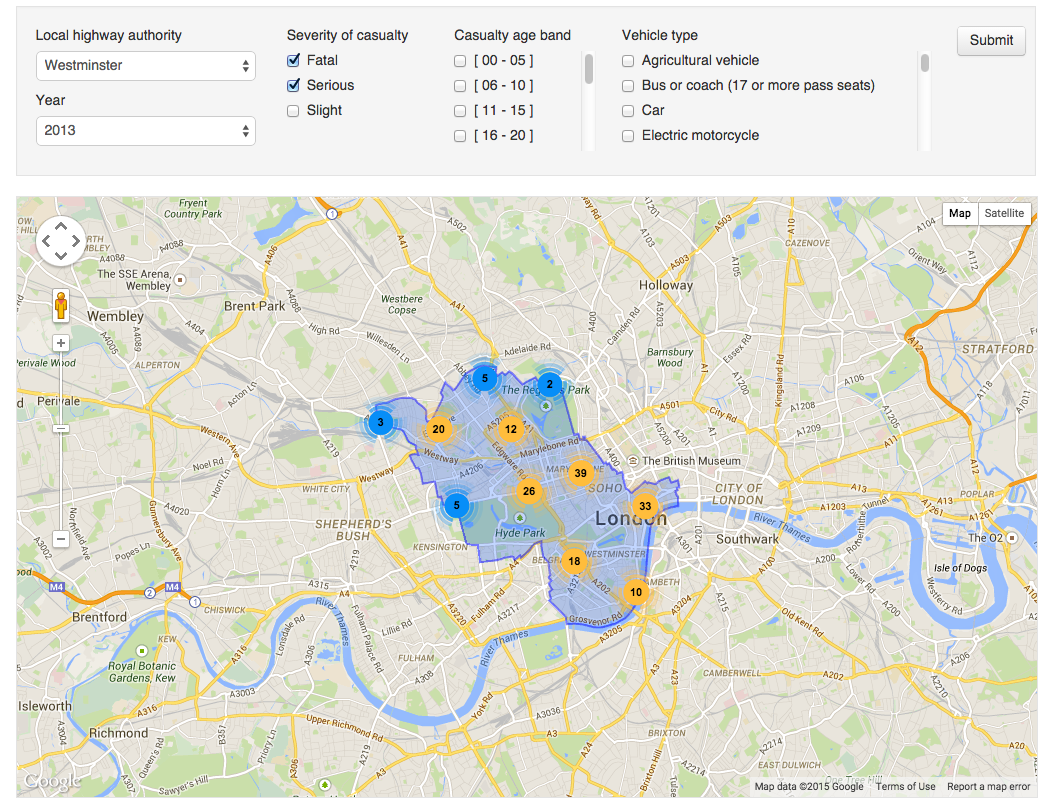
\includegraphics[scale=0.3]{collisionmap}
	\caption{Collision Map application}
	\label{fig:collisionmap}
\end{figure}

Motorcycle Accidents \citep{Mceinsurance} provides an interactive guide to motorcycle accidents in the UK. The aim of this application is to provide motorcyclists with information about where and when it is safest to ride. The application allows you to view statistics about motorcycle accidents on a regional basis (see \autoref{fig:motorcycle}). The application makes use of several fields from the open datasets, including road conditions, time of day and severity. For each field, you can view a break down of the data in each region. For example, you can analyse how accidents depend on time of day in London. The application also presents two key facts for each field in order to summarise the data.

The data is presented in a manner that is easy to analyse for any user, and the facts give a concise summary of the findings from the data. This is adequate to serve the application's purpose, but there are limitations that affect the overall usefulness. For example, it isn't possible to view specific accident hotspots. The regions cover very large areas, and there is no breakdown of where the accidents occur within these areas.

\begin{figure}
	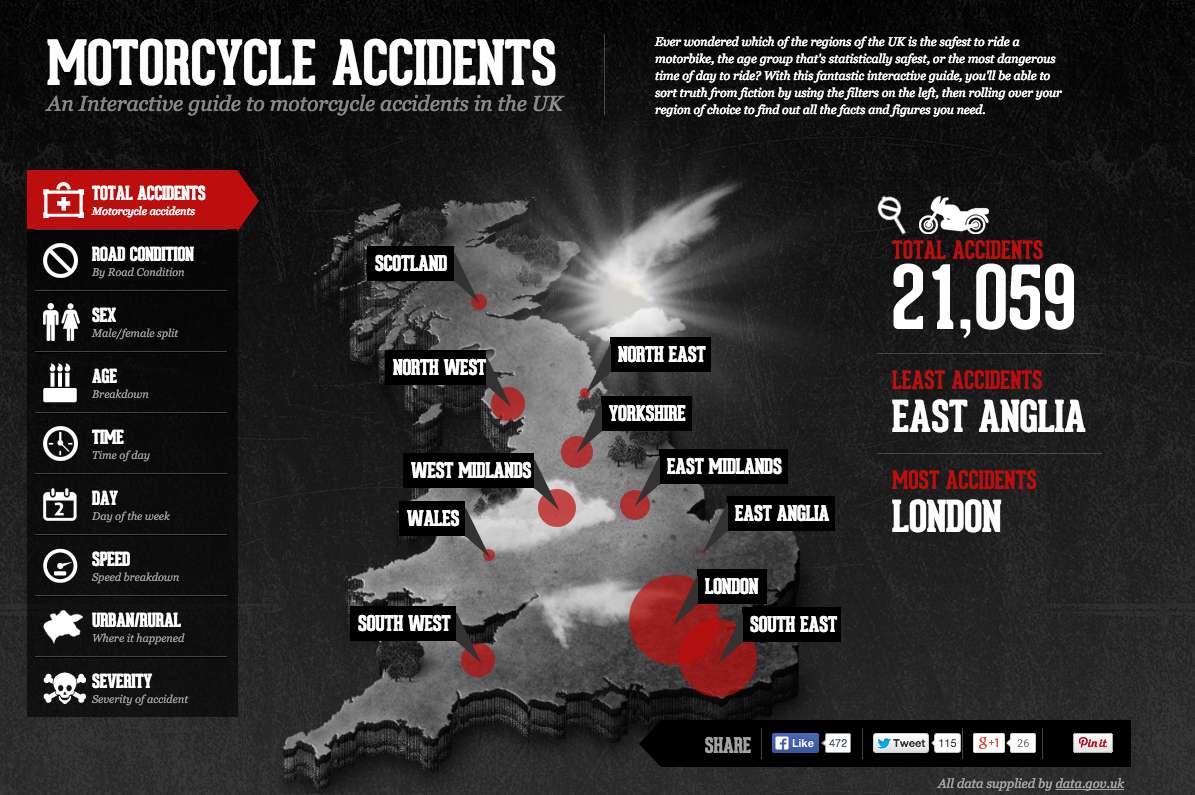
\includegraphics[scale=0.3]{motorcycle}
	\caption{Motorcycle Accidents application}
	\label{fig:motorcycle}
\end{figure}

The final application that I will look at is Walkonomics \citep{Davies}. Walkonomics aims to rate the 'walkability' of streets around the world by combining the views of large groups of people, local communities and open data. You can search for a location, and the application will return a list of streets near that location, along with a map displaying markers for each street (see \autoref{fig:walkonomics}). You can then click on a street name in order to find out more information about that street. This page presents a list of reviews for that street, including one from 'Walkobot' which is based on various open datasets. Additionally, a user may add a review of their own on this page. 

Walkonomics extends what the other applications have achieved with open data. Not only does it use open data from different countries, but it also uses different types of data (road safety and crime are mentioned). In addition to this, it combines the use of open data with crowdsourcing. Beyond being a web application, Walkonomics is also available to download as an App on both Android and iOS devices.

However, there are some major limitations to this application. For example, when searching for several major cities across the world (including Cardiff, Edinburgh, Paris, Sydney and Los Angeles), no results are found. It is unclear whether this is a bug or expected behaviour. Additionally, there is no transparency over which open datasets are used; it mentions the use of road safety and crime data, but doesn't specify which countries/states they have obtained this data from. As an application that claims to use data from various different sectors and sources, it should provide a more detailed list of datasets used.

\begin{figure}
	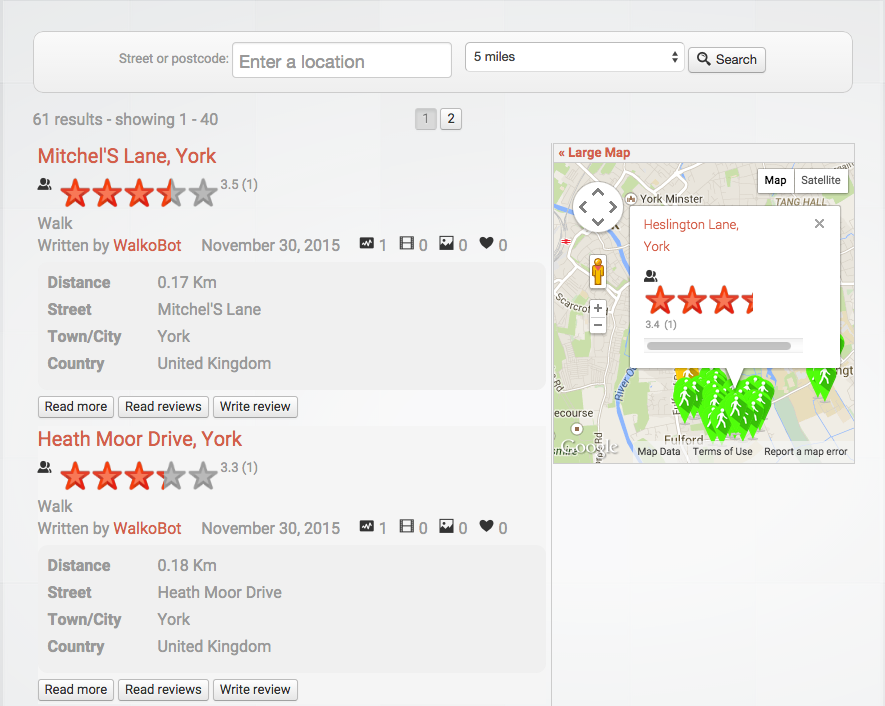
\includegraphics[scale=0.4]{walkonomics}
	\caption{Walkonomics application}
	\label{fig:walkonomics}
\end{figure}

A comparison of some properties of these four applications can be seen in \autoref{tab:applications}. It is immediately apparent that none of the applications are open source. As these applications rely on open data, it is disappointing that the developers do not want their code to be open. The community would benefit greatly from this, as people like myself looking to build new applications would be able to more thoroughly analyse the existing work. By sharing ideas about how to develop such applications, the community can work together to improve them and agree on the best approach.

Another noticeable aspect from this comparison is the similarities between Crash Map and Collision Map. In fact, there are several other applications listed on \textit{data.gov.uk} that are similar to these. This led to the Department for Transport taking Collision Map offline in March 2015, as they felt it offered low value to taxpayers due to the number of alternatives available.  All of these applications operate in the same way; you zoom to an area of the map, and all accidents within that area are displayed. There are no advanced searching facilities available, such as searching for accidents on a particular route only. If you wanted to find such information, you would need to find the route yourself and manually pan the map, counting how many accidents are plotted. Clearly there is room for a new application that provides more advanced features like this.  


\begin{table}[tbp]
  \centering
  \begin{tabular}{ p{2.5cm}  p{3.2cm}  p{2.2cm}  p{2.2cm} }
      \textbf{Application} & \textbf{Data} & \textbf{Platform(s)} & \textbf{Open Source?} 
    \\Crash Map & UK Road Safety 05-13 & Web & No
	\\Collision Map & UK Road Safety 05-13 & Web & No
	\\Motorcycle Accidents & UK Road Safety 11-13 (motorcycle only) & Web & No
	\\Walkonomics & Road Safety, Crime & Web, iOS, Android & No
  \end{tabular}
  \caption{Comparison of applications that use road safety data}
  \label{tab:applications}
\end{table}

\subsection{Research in Open Data}

\section{Web Application Development}

\subsection{Overview}

Jazayeri's paper, 'Some trends in web application development', discusses the area of web application development from a software engineering perspective \citep{Jazayeri2007}. The Web is described as "an attractive playground for software engineers where you can quickly release an application to millions of users and receive instant feedback". It is argued that web applications reach "users that are varied in age, culture, language, education, interest, needs, etc.", and that providing for such varied users poses many interesting challenges. However, whilst all applications may be able to reach such a varied audience, I would argue that most have a specific target audience that the application can be catered to. Hence the challenges of providing for a varied user base is more dependent on the type of application, rather than the platform on which the application is available. 

A major benefit of web applications over desktop applications is the ease in which new versions can be released. In a desktop application, even a small bug fix will require a new version to be installed for all clients. This can lead to numerous issues, as explained by Jazayeri \citep{Jazayeri2007}. In contrast, a web application exists on one server and the browser acts as a universal client. This means that features and bug fixes can be deployed as soon as they are ready, and users will instantly have access to the upgraded application without having to install an update. This leads more kindly to an agile development strategy, as small updates can be released at any time with no impact on users. Desktop applications are more likely to require updates to be grouped together in order to reduce the number of updates that the user must install. However, it is worth noting that some web applications may also require updates to be bundled if they require downtime in order to be applied.  

Web development has been "driven by a move towards open source and standardised components" \citep{Jazayeri2007}. This trend is seen right through web development, from the application itself to the server that it is hosted on. The standard open source server environment used by many is commonly referred to as LAMP. This represents the operating system (Linux), the web server (Apache), the database server (MySQL), and the scripting language (PHP, Perl or Python). An example of a typical LAMP architecture can be seen in figure x. The main advantage of a  LAMP environment is that it can be assembled relatively easily and cheaply. PHP, MySQL and Apache are the three most commonly used tools in their respective categories. They have all been developed by programmers within the community who focus on writing features that they want and need \citep{Nixon2009}. As the code is available for all to see and change bugs can be resolved and potential security issues can be prevented before they happen.


\subsection{Programming Languages}

In this section I will compare and contrast some of the most popular programming languages used for web applications. I will focus on three of the most popular server-side scripting languages that are used in modern web applications; PHP, Python and Ruby. I will also look at the most popular client-side scripting language, JavaScript.

PHP is a server scripting language designed by Rasmus Lerforf. It is fast, flexible and one of the most popular scripting languages available. According to Netcraft's Web Server Survey of January 2013, PHP was being used by 244M sites at this time \citep{Ide2013}. This equates to 39\% of all sites used in the survey. A large factor behind this popularity is the number of content management systems and ecommerce solutions that are written in PHP; WordPress, Joomla, Drupal, Zencart, osCommerce and Megento account for 32M of these sites. PHP's main advantages include the number of built-in libraries for common web tasks, the ease of learning and use, and its portability \citep{Welling2005}. Its flexible integration with HTML makes client tier integration easy. The main disadvantage of PHP stems from its huge popularity. Because of the huge number of applications authored in PHP, hackers are presented with a "huge and rather attractive attack surface" \citep{Ide2013}. Additionally, due to the open source nature of PHP, it is easier for hackers to find exploits. 

Ruby is a dynamic, imperative object-oriented programming language developed by Yukihiro Matsumoto. Ruby on Rails is a popular framework for web application development based on the model view controller pattern. This framework adds a set of powerful functionalities such as scaffolding, active record, migrations, routing, environments, and many helper functions \citep{Jazayeri2007}. Advantages of Ruby include better security features, pure object-oriented programming, highly readable code and good testing frameworks. Disadvantages include a steep learning curve and a lack of informational resources.

Python was first released in 1991 by Guido van Rossum. In contrast to PHP, it was initially designed as a full-featured general purpose language. It supports multiple programming paradigms, including object-oriented and functional programming. Its design philosophy emphases code readability. Python is quick and easy to learn and it has a large community who provide good support. Disadvantages of Python include its lack of true multiprocessor support and absence of commercial support. 

Klaus Purer directly compares these three scripting languages in 'PHP vs. Python vs. Ruby - The web scripting language shootout' \citep{Purer2009}. In this paper, Purer aims to compare the languages objectively, using only facts rather than opinion. The first metric used to compare the languages is popularity, which is notoriously difficult to measure. Purer concludes that PHP is the most popular, followed by Python, with Ruby the least popular. This is based on search engine ratings, availability on hosting providers and discussion media ratings. It would have been interesting to include some additional metrics, such as the frequency in which the languages feature in GitHub repositories. GitHut is an online tool that visualises this data \citep{Zapponi2014}. It shows that in Q4 of 2014, Python featured in the most active repositories, with PHP second, and Ruby third. Whilst this suggests that the relative popularity may have changed since Purer's report of 2009, the TIOBE Index for March 2015 still shows PHP above Python \citep{TIOBESoftware2015}. 

Purer goes on to compare the readability and usability of these languages. Once again this is difficult to measure scientifically. He states that PHP follows a "very classical approach" and will feel very familiar to former C-programmers, Python's strict indentation enforcements and small set of keywords make it suitable for programming beginners, and Ruby will be attractive for experienced programmers looking for "elegant and powerful programming expressiveness". He concludes that Python is the most readable due to its enforced program structure and Ruby is the most usable because of its "principle of least surprise". Whilst these conclusions seem valid, personal preference will have had an influence due to the unquantifiable nature of usability and readability. 

In the next section, Purer compares some features of the three languages, including exception handling, database abstraction, functional language features, interactive development  with the interpreter and duck typing. It is argued that PHP has inferior exception handling as it was only added in version 5, meaning that some content management systems and frameworks lacked proper exception support in their code. As the report is focused on comparing the languages, I would argue that it is unfair to criticise PHP for a feature that it provides because it hasn't been utilised by some developers. A similar criticism is made of PHP regarding relational database abstraction. It is put forward that PHP is "a little bit behind the other two languages, as the abstraction has not been adapted by long-living PHP projects". I believe that an unbiased comparison of the three languages should focus purely on the features of the languages, rather than the implementation of the features by some developers. Additionally, no evidence is provided to back up these claims. 

In the final sections, Purer compares the security and performance of the languages. It is concluded that the performance levels of the languages are very similar, and PHP is slightly inferior to the other languages in terms of security. PHP is mainly criticised for allowing poor programming practices which "result in many security related bugs". This is a valid criticism, but it is also worth noting that a skilled developer can create a secure PHP application. 

Overall, this paper provides an interesting discussion and some useful information about the languages involved. As acknowledged by the author, choosing a programming language is often connected to personal experience and discussions can therefore be irrational. Whilst Purer tried to avoid this, it seems apparent that some of his conclusions are slightly irrational and not based on facts. Most features compared weren't quantifiable, making it very difficult to draw conclusions without some bias.

Client-side JavaScript combines "the scripting ability of a JavaScript interpreter with the Document Object Model (DOM) defined by a web browser" \citep{Flanagan2006a}.This means that it can add behaviour to otherwise static web content. This technology is the core of web development techniques such as Dynamic HTML and architectures such as Ajax (Asynchronous JavaScript and XML). JavaScript helps reduce server usage, as functions that were typically performed on the server can be done on the client (e.g. form validation) \citep{Jazayeri2007}. Browsers are able to provide more responsive operations to the user by pushing some of the client-server communication to the background while the application is still interactive. This can be achieved using Ajax to introduce an intermediary 'engine' between the user and the server \citep{Garrett2005}. Every user action that would normally generate a HTTP request takes the form of a JavaScript call to the Ajax engine instead. If the engine needs something from the server to respond (e.g. retrieving new data), the engine makes those requests to the server asynchronously without interrupting the user's interaction with the application. 


\subsection{Model-View-Controller}

A large number of contemporary web frameworks make use of the Model-View-Controller (MVC) design pattern. The Model is the application object, the View is its screen representation, and the Controller defines the way the user interface reacts to user input \citep{Gamma1995}. The MVC pattern had been popular in software engineering for many years before it was realised that it could be applied just as well to web applications \citep{Jazayeri2007}.  The main problem with using the MVC design pattern when developing web applications is that the application must be partitioned between the client and the server \citep{Leff2001}.

Morales-Chapar et al. provide an interesting discussion on the different implementations of MVC in web applications \citep{Morales-Chaparro2007}. This paper focuses on "large-scale web applications which are data dynamic and typically written in two programming languages", much like my application will be. A case study is used to compare the advantages and disadvantages of server-side MVC with two mixed client-side and server-side MVCs. 

Server-side MVC is derived from desktop MVC, in that all components are usually programmed in the same language and the server runs all computations and operations. It is pointed out by Morales-Chaper et al. that this approach is useful when "applications capabilities requirements are poor at client side (e.g. mobile browsers without JavaScript functionality) or when application necessity is only to display information with low levels of user interaction". It is worth consideration that this paper was published in 2007, and since this time mobile devices and browsers have advanced significantly, so the first advantage given is of little relevance now. The disadvantages of this approach include the incapability of updating part of a view, increased bandwidth usage and the higher server usage due to the server validating forms, amongst other things.  

The first mixed client-side and server-side MVC discussed by Morales-Chapar et al. was designed with a focus on resolving the previously raised issues. This MVC design involves dividing the Controller and View between the server and client, whilst leaving the model at server-side. In this system, some processing is now done on the client-side; for example, form validation using JavaScript. They raise the issue of different browsers and operating systems causing issues when accessing UI elements. Whilst the situation has improved since 2007, there still exists the issue of browsers not implementing exactly the same standard specifications. This approach still has the disadvantage of not being able to retrieve data asynchronously without refreshing the page. Without a model on the client-side, there are limitations on providing high interaction levels and data manipulation becomes more difficult. In comparison with the pure server-side approach, there is an increase in computation time and complexity due to the logic now present on client-side. 

The second mixed client-side and server-side MVC discussed by Morales-Chapar et al. is similar to the previous design, but with part of the model on client-side. This design addresses the issue of not being able to retrieve data asynchronously without refreshing the page, by allowing for the use of Ajax. Limitations of this design include slower computation for tasks requiring access to the server, difficulty of designing a client-side model that is compatible with all browsers, and increased overhead on communications among MVC design elements. 


\section{Software Development Methodologies}

In this section, I will discuss some popular software engineering methodologies that I will consider using for this project. I will focus on those that are most beneficial to a project like this one, i.e. a web application developed by one person in a limited time frame. 

Pfleeger and Atlee define software engineering as “an approach that combines computer science (which is made up of theories and computer functions) and the customer (who provides the problem to be solved) to develop a set of tools and techniques to solve problems” [1]. Software engineering methodologies can be defined as a group of methodologies used in the development of applications. Methodologies give details of “what should be done in each phase of the software development process” [2]. They do not necessarily give details of how things should be done, allowing for some tuning by those using them. 

Agile software development is a conceptual framework for undertaking software engineering projects [3]. Agile methods generally try to minimise risk by developing software in iterations, which typically last one to four weeks. Each iteration of the project is like its own project, featuring its own planning, requirement analysis, design, coding, testing and documentation phases. At the end of each iteration, a new working version of the application should be available. The team is then able to reevaluate the project priorities ahead of the next iteration. Agile methods emphasise working software as a primary measure of progress.

Scrum is a software-management process for iterative-incremental software development projects. Scrum relies on self-organisation, with the team deciding what to do while management removes roadblocks [4]. Scrum is focused on frequent intermediate delivers with working functionality. Alongside this, there are frequent risk and mitigation plans produced by the development team. There are daily ‘scrums’, where the development team meetup to explain progress, describe upcoming work and raise obstacles. 

Extreme Programming is an iterative and incremental development methodology. Key practices of Extreme Programming include making a rough plan quickly and refining it as thing become clearer, test driven development, refactoring code, continuous integration of code and an on-site customer to clarify requirements and make crucial business decisions [4]. 


\section{Usability of Interactive Applications}

\chapter{Requirements Analysis}

\section{Functional Requirements}

\begin{tabular}{| p{2.2cm} | p{7.5cm} | p{2cm} |}
	\hline
	\textbf{Requirement ID} & \textbf{Description} & \textbf{Importance} \\ \hline
	FR1 & The application should use road safety data published by the UK Department for Transport to warn users about accident hotspots. & High \\ \hline
	FR2 & Users should be able to specify road journeys, and the road safety data should be used to highlight risks on the selected route. & High \\ \hline
	FR3 & Users should be able to specify time of travel in order to further filter the data. & Medium \\ \hline
	FR4 & Users should be able to set warning thresholds, such as frequency and severity of accidents. & Medium \\ \hline
	FR5 & Users should be able to specify weather conditions in order to further filter the data. & Low \\ \hline
	FR6 & Weather data should be retrieved from the Met Office DataPoint service using the location and time parameters specified by the user. This data should then be used to filter the road safety data. & Low \\ \hline
	FR7 & The application should suggest lower risk routes for the specified journey. & Low \\ \hline
	FR8 & The location of incidents should be displayed on an interactive map. & High \\ \hline
	FR9 & Users should be able to retrieve additional information about an incident. & Medium \\ \hline
	FR10 & UThe application should be compatible with the latest versions of Google Chrome, Mozilla Firefox and Internet Explorer. & High \\ \hline
	FR11 & The application should be compatible with mobile devices. & Low \\ \hline
	FR12 & The site administrator should be able to add and remove datasets through a user-friendly GUI. & High \\ \hline
	FR13 & The road safety data should be automatically updated when new datasets are released. & Low \\ \hline
	FR14 & A generic ‘boilerplate’ implementation should be developed that can be reused to develop other Open Data applications. & Medium \\
	\hline
\end{tabular}

\section{Non-functional Requirements}

\begin{tabular}{| p{2.2cm} | p{7.5cm} | p{2cm} |}
	\hline
	\textbf{Requirement ID} & \textbf{Description} & \textbf{Importance} \\ \hline
	NFR1 & The results of any data analysis should be presented in a user-friendly way. & High \\ \hline
	NFR2 & The response time of the application should be <5 seconds, assuming that the user's connection isn't the bottleneck. & High \\ \hline
	NFR3 & The user interface should use standard controls. & Medium \\
	\hline
\end{tabular}


\chapter{Design}

\section{System Architecture}

\subsection{LAMP}

\subsection{UML Diagram}

\section{Development Process}

\section{Technology Overview}

\subsection{PHP}

\subsection{MySQL}

\subsection{Google Maps API}

\subsection{Version Control System}

\section{Interface Design}

\subsection{Wireframes}

\section{Summary}

\chapter{Implementation and Testing}

\section{Components}

\section{Techniques}

\section{Testing}

\section{Summary}

\chapter{Evaluation}

\section{Discussion}

\section{Usability}

\section{Maintainability}

\section{Limitations}

\chapter{Conclusions}

\section{Lessons Learnt}

\section{Future Work}


\bibliography{library}


\end{document}
